\section{Supersafety to Perfect Timeliness}

We now construct a perfectly timely protocol $\bar\Pi$
using a black-box reduction from a supersafe, and live($u$) protocol $\Pi^*$.
Each honest party $P$, executing the $\Pi^*$ protocol, runs a
full node of protocol $\Pi$.
The ledger of party $P$ for protocol $\Pi$ and $\Pi^*$ is denoted as $\Ledger[][\Pi][r]$ and
$\Ledger[*][\Pi][r]$ respectively.
The main idea is that new transactions appearing in $\Ledger[][][r]$ are
concatenated with $\Ledger[*][][r - 1]$ and reported
with recorded round $r$
to create temporal ledger $\Ledger[*][][r]$.
This process is illustrated
in Figure~\ref{fig:backward-reduction}
and the pseudocode is presented in Algorithm~\ref{alg:backward-reduction}.

\begin{figure}
  \centering
  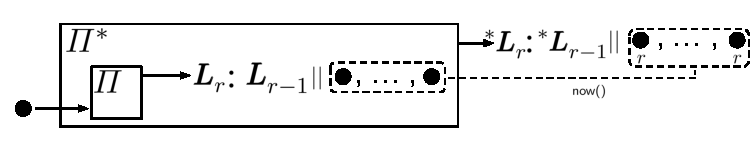
\includegraphics[width=0.9\columnwidth,keepaspectratio]{figures/backward-reduction.pdf}
  \caption{The reduction from Supersafety
    (the $\Pi$ protocol) to Perfect Timeliness (the $\Pi^*$ protocol).
  }
 \label{fig:backward-reduction}
\end{figure}

\import{./}{algorithms/algorithm-backward-reduction.tex}

\dznote{Describe and prove the reverse reduction}
